\documentclass[15pt,t,aspectratio=1610]{beamer}

%%% INCLUDE TEX SETUP
\usepackage[german]{babel}
\usepackage[latin1]{inputenc}
\usepackage{csquotes}
\usepackage{times}
\usepackage{txfonts}
\usepackage{amsmath}
\usepackage{amsfonts}
\usepackage{upgreek}
\usepackage{amssymb}
\usepackage{multimedia}
\usepackage{rotating}
\usepackage{graphicx}
\usepackage{xy}
\usepackage{paralist}
\usepackage{pdfpages}
% \usepackage[autoplay,every=1,type=png]{animate} % \usepackage[every=1]{animate}
\usepackage{pdfanim}
\setlength{\fboxrule}{5pt}
\usepackage{tikz}
\usetikzlibrary{arrows,decorations.pathmorphing,backgrounds,positioning,fit,petri,shapes,topaths}
\usetikzlibrary{calc}
\usepackage{multirow}

\usepackage{tensor}
\usepackage{multicol}

% %%%%%%%%%%%%%%%%%%%%%%%%%%%%%%%%%%%%%%%%%%%%%%% USER DEFINED COMMANDS AND PATHS %%%%%%%%%%%%%%%%%%%%%%%%%%%%%%%%%%
\newcommand{\insertpicture}[2]{\begin{minipage}{#1}\centering\includegraphics[width=\textwidth]{#2}\end{minipage}}
%%%%%%%%%%%%%%%%%%%%%%%%%%%%%%%%%%%%%%%%%%%%%%% COLOR DEFINITIONS %%%%%%%%%%%%%%%%%%%%%%%%%%%%%%%%%%%%%%%%%%%%%%%%
\definecolor{tublue}{rgb}{0.04,0.16,0.32}
\definecolor{greycust}{rgb}{0.50,0.50,0.50}
\definecolor{gwhite}{rgb}{0.99,0.99,0.99}
\definecolor{tubluelight}{rgb}{0.12,0.45,0.87}
\definecolor{altcol}{rgb}{0.8,0.0,0.0}      % AlertColor
\definecolor{mygray}{gray}{0.8}
\definecolor{mygray2}{gray}{0.6}
\definecolor{headgray}{gray}{0.4}
\newcommand{\red}{\color{red}}
\newcommand{\black}{\color{black}}
\newcommand{\tublue}{\color{tublue}}
\setbeamercolor{normal text}{fg=tublue}%
\setbeamercolor{structure}{fg=tublue}%
\setbeamercolor{alerted text}{fg=tubluelight}%
\setbeamercolor{section in toc}{fg=tublue}%
\setbeamercolor{item}{fg=tubluelight}%
\setbeamercolor{block title}{fg=tubluelight}%
\setbeamercolor{footline}{fg=greycust}
\setbeamercolor{background canvas}{bg=}
%%%%%%%%%%%%%%%%%%%%%%%%%%%%%%%%%%%%%%%%%%%%%%% TITLE CONFIGURATION %%%%%%%%%%%%%%%%%%%%%%%%%%%%%%%%%%%%%%%%%%%%%%
\newcommand{\nframetitle}[1]{\frametitle{\hspace{9.4mm}\textcolor{tublue}{#1}}\vspace{-8mm}\vfill} % \put(3.5,4.8){\tiny \textbf{Department of Mathematics~}Institute of Scientific Computing}
\newcommand{\newframesubtitle}[1]{\framesubtitle{\hspace{7mm} \textcolor{tublue}{#1}}}
\newcommand{\newframesubtitletwo}[1]{\frametitle{\centering \Large #1}}
%%%%%%%%%%%%%%%%%%%%%%%%%%%%%%%%%%%%%%%%%%%%%%% HEADLINE %%%%%%%%%%%%%%%%%%%%%%%%%%%%%%%%%%%%%%%%%%%%%%%%%%%%%%%%%
\setbeamertemplate{navigation symbols}{}
\useoutertheme[hoptionsi]{miniframes}

% HEADER STYLE (16:10)
\setbeamertemplate{headline}{
	\begin{beamercolorbox}{section in head}
		\vskip4pt
		%%% TU LOGO
		\begin{minipage}{33.5mm}
			{\rule{2.5mm}{0pt}\rule[-0.5mm]{0pt}{3.5mm}
\includegraphics[width=30mm]{pic/logo/tu_blau.pdf}}
		\end{minipage}
		\hfill
		%%% NAVIGATION ITEMS
		\begin{minipage}{85mm} % ADJUST THE WIDTH OF THIS MINIPAGE TO YOUR CONTENT
			{\rule{4.5mm}{0pt}\insertnavigation{83mm}} % AND THIS
		\end{minipage}
		\hfill
		%%% ADDITIONAL LOGO (if needed)
		\begin{minipage}{15mm}
			{\rule{2.5mm}{0pt}
			%\includegraphics[height=10mm]{logo_ilr.pdf}
		}
		\end{minipage}
		\vskip2pt
		% DIVIDER BETWEEN HEADER AND CONTENT (TWO LINES)
		\begin{minipage}{128mm}
			\setlength{\unitlength}{1mm}
			\begin{picture}(128,1.5)
			\linethickness{.1mm} \put(-10,1.3){\line(1,0){175}}
			\linethickness{.1mm} \put(-10,0){\line(1,0){175}}
			\end{picture}
		\end{minipage}
	\end{beamercolorbox}
} % 197.2 x 166.5
% FOOTER STYLE
\setbeamertemplate{footline}{
	\vfill
	\vspace{-10mm}
	\begin{minipage}{\textwidth}
		\rule{\textwidth}{.1mm}
		\vskip2pt 
		$\quad$\tiny Institute of Scientific Computing 
		\hfill
		\insertframenumber%\inserttotalframenumber
		$\quad$\\
		\vskip3pt
	\end{minipage}
}
\setbeamersize{text margin left=12.9mm,text margin right=12.9mm}

% Bibliography
\usepackage[backend=bibtex,style=alphabetic,language=american]{biblatex}
\bibliography{lib}
\usepackage[draft]{todonotes}   % notes showed

%% FOOTNOTE INDENTATION
\makeatletter
%\renewcommand\@makefntext[1]{\leftskip=2em\hskip-2em\@makefnmark#1}
\renewcommand\@makefntext[1]{\leftskip=10pt\hskip-3.7pt\@makefnmark#1}
\makeatother

% user commands 
\newcommand{\eg}{e.\,g.}%
\newcommand{\formComma}{\,\text{,}}
\newcommand{\formPeriod}{\,\text{.}}
\newcommand{\R}{\mathbb{R}}%
\newcommand{\xb}{\mathbf{x}}%
\newcommand{\ub}{\mathbf{u}}%
\newcommand{\tub}{\tilde{\ub}}%
\newcommand{\tu}{\tilde{u}}%
\newcommand{\vb}{\mathbf{v}}%
\newcommand{\eb}{\mathbf{e}}%
\newcommand{\gb}{\mathbf{g}}%
\newcommand{\Xb}{\mathbf{x}}% parametrization X:{(theta,phi)} --> R3
\newcommand{\fv}{\underline{\mathbf{f}}}
\newcommand{\pv}{\underline{\mathbf{p}}}
\newcommand{\scalarprod}[1]{\big\langle{#1}\big\rangle}%
\newcommand{\exd}{\mathbf{d}} %exterior derivative
\newcommand{\lie}{\mathcal{L}} %Lie-Ableitung
\newcommand{\surf}{\mathcal{S}}
\newcommand{\gaussianCurvature}{\kappa}
\newcommand{\Grad}{\operatorname{grad}}
\newcommand{\Div}{\operatorname{div}}%
\newcommand{\Rot}{\operatorname{rot}}%
\newcommand{\DivSurf}{\Div_{\surf}}%
\newcommand{\GradSurf}{\Grad_{\surf}}
\newcommand{\RotSurf}{\Rot_{\surf}}
\newcommand{\laplaceBeltrami}{\Delta_{\surf}}
\newcommand{\vecLaplace}{\boldsymbol{\Delta}}
\newcommand{\laplaceDeRham}{\vecLaplace^{\textup{dR}}}
\newcommand{\laplaceRotRot}{\vecLaplace^{\textup{RR}}}
\newcommand{\laplaceGradDiv}{\vecLaplace^{\textup{GD}}}
\newcommand{\LaplaceDeRham}{Laplace-deRham }
\newcommand{\ProjectSurf}{\pi_\surf}
\newcommand{\Tangent}{\mathsf{T}}
\newcommand{\vect}[1]{\mathbf{#1}}
\newcommand{\landau}{\mathcal{O}} %landau symbol O
\newcommand{\SC}{\mathcal{K}} % simplicial complex
\newcommand{\Vs}{\mathcal{V}} % set of vertices
\newcommand{\Es}{\mathcal{E}} % set of edges
\newcommand{\Fs}{\mathcal{T}} % set of faces
\newcommand{\face}{T} % one face
\newcommand{\FormSpace}{\Lambda^{1}} % space of 1 forms
\newcommand{\U}{u} %Komponenten des Geschwindigkeitfeldes
\newcommand{\Ub}{\mathbf{\U}} %Geschwindigkeitsfeld
\newcommand{\tU}{\tilde{u}} %Komponenten des Geschwindigkeitfeldes
\newcommand{\tUb}{\mathbf{\tU}} %Geschwindigkeitsfeld
\newcommand{\lc}{\mathbf{E}} % Levi-Civita-Tensor



\begin{document}

	%%% TITLEPAGE
	\setbeamercolor{background canvas}{bg=tublue}
\begin{frame}
%%%%%%%%%%% TITLE PAGE %%%%%%%%%%%%%%%%%%%%%%%%%%%%%%%%%%%%%%%%%%%%%%%%%%%%%%%%%%%%%%%%%%%%
% 16:10
\Large{
	\vspace{-12mm}
	\hspace{-8mm}
	\begin{minipage}{33.5mm}
		
\includegraphics[width=30mm]{pic/logo/tu_weiss.pdf}
	\end{minipage}\\
% 	\hfill
	\textcolor[rgb]{1.00,1.00,1.00}{
		\begin{minipage}{163mm}%{228mm}
			\setlength{\unitlength}{1mm}
			\begin{picture}(148,8)
				\linethickness{.1mm} \put(-15,7){\line(1,0){165}}
				\put(3.4,4.8){\tiny \textbf{Department of Mathematics~}Institute of Scientific Computing}
				\linethickness{.1mm} \put(-15,4){\line(1,0){165}}
			\end{picture}
		\end{minipage}
		\rule{0pt}{2.3em}
		\begin{center}
			{\huge \textbf{Discrete Exterior Calculus (DEC) for the
      Surface Navier-Stokes Equation}}
		\end{center}
		\rule{0pt}{3.7em}
		\begin{center}
			{\small Ingo Nitschke\\} %\rule{0pt}{1em}%\vspace{1em}
			{\footnotesize \emph{Institute of Scientific Computing}} \\
		\end{center}
		\rule{0pt}{5em}
% 		\tikz[overlay,remember picture]
% 		\node[anchor=center] at ($(current page.center)+(6,-2.5)$) {
% 			{\tiny\emph{Financial support provided by}}
% 		};
% 		\tikz[overlay,remember picture]
% 		\node[anchor=center] at ($(current page.center)+(6,-3.6)$) {
% 			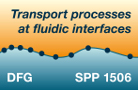
\includegraphics[width=0.2\textwidth]{pic/logo/spp1506.jpg}
% 		};
% 		\tikz[overlay,remember picture]
% 		\node[anchor=center] at ($(current page.center)+(-6,-3.6)$) {
% 			\includegraphics[width=0.2\textwidth]{pic/logo/logo_dfg.jpg}
% 		};
	}
	\thispagestyle{empty}
}

\end{frame}
\setbeamercolor{background canvas}{bg=}


	%%% TABLE OF CONTENTS 
	\begin{frame}
		\nframetitle{Content}
		\tableofcontents
	\end{frame}

  \section{Motivation}
	\begin{frame}
		\nframetitle{Content}
		\tableofcontents[current]
	\end{frame}

  \begin{frame}
    \nframetitle{Navier-Stokes Equation\footnotemark[1]}
    \begin{itemize}
      \item Smooth Riemannian surface \( \surf \) without boundary
      \item Inextensible homogeneous medium
      \item No external forces
      \item Tangential surface velocity field: \( \vb(t)\in\Tangent\surf \)
      \item Conservation of mass:\quad \( \Div\vb = 0 \)
      \item Conservation of linear momentum:\quad \( \rho\left(\partial_{t}\vb + \nabla_{\vb}\vb\right) = \Div\mathbf{\sigma} \)
      \item Surface Cauchy stress tensor:
            \( \tensor[^{\flat}]{\mathbf{\sigma}}{^{\flat}} = -p\gb + \mu\lie_{\vb}\gb \)
      \item \( \Rightarrow\quad \partial_{t}\vb + \nabla_{\vb} \vb = - \Grad p + \frac{1}{\text{Re}} \left(- \laplaceDeRham \vb + 2 \gaussianCurvature \vb \right)\)
      \item Laplace-DeRham:\quad \(- \laplaceDeRham \vb = \Div\Grad\vb - \gaussianCurvature \vb  \) \quad (Weitzenb"ock)
    \end{itemize}
		\vskip10pt
		\footnotetext[1]{\tiny\fullcite{ArroyoDeSimone_PRE_2009}\vskip0pt}
  \end{frame}

  \begin{frame}
    \nframetitle{Vorticity Equation}
          \begin{align}
            \begin{aligned}
            \partial_{t}\vb + \nabla_{\vb} \vb &= - \Grad p + \frac{1}{\text{Re}} \left(- \laplaceDeRham \vb + 2 \gaussianCurvature \vb \right)
              &\text{and}&&\Div\vb &= 0
              \end{aligned}\tag{NSE}
          \end{align}
    \begin{itemize}
      \item Streamfunction: \( \psi \) with \( \vb = \Rot\psi \)
      \item Vorticity: \( \Rot\vb = \Delta\psi \)
      \item Applying \( \Rot \) on (NSE): 
        \begin{align}
          \partial_{t}\Delta\psi + \left\langle \Rot\psi , \Grad\Delta\psi \right\rangle &= \frac{1}{\text{Re}}\left( \Delta^{2}\psi + 2\Div\left( \gaussianCurvature\Grad\psi \right) \right)
          \tag{VE}
        \end{align}
      \item Approaches:\quad \eg 
        \begin{itemize}
          \item Surface Finite Element Method\footnotemark[1]\footnotemark[2] (SFEM)
          %\item Diffuse Interface\footnotemark[3]\footnotemark[4] (DI)
          \item Diffuse Interface\footnotemark[3] (DI)
            \item Discrete Exterior Calculus (DEC)
        \end{itemize}
    \end{itemize}
		\vskip5pt
		\footnotetext[1]{\tiny\fullcite{Nitschkeetal_JFM_2012}}
		\footnotetext[2]{\tiny\fullcite{Reutheretal_MMS_2015}}
		%\footnotetext[3]{\tiny\fullcite{Raetzetal_CMS_2006}}
		\footnotetext[3]{\tiny\fullcite{Reutheretal_JCP_2016}\vskip0pt}
  \end{frame}

  \begin{frame}
    \nframetitle{Vorticity Equation}
        \begin{align}
          \partial_{t}\Delta\psi + \left\langle \Rot\psi , \Grad\Delta\psi \right\rangle &= \frac{1}{\text{Re}}\left( \Delta^{2}\psi + 2\Div\left( \gaussianCurvature\Grad\psi \right) \right)
          \tag{VE}
        \end{align}
    \begin{itemize}
      \item \textbf{Drawback}: reduced solution space for genus \( g(\surf)\ne 0 \)  (\eg\ Torus)
      \item Hodge decomposition:\quad
            \( \vb = \Rot\psi + \Grad\varphi + \vb_{\text{Harm}}  \)
      \item Harmonic vector field \( \vb_{\text{Harm}}\in\Tangent_{\text{Harm}}\surf \):\quad
            \( \Div\vb_{\text{Harm}} = \Rot\vb_{\text{Harm}} = 0 \)
      \item For \( g(\surf)\ne 0 \):\quad \( \operatorname{dim}_{\R}\Tangent_{\text{Harm}}\surf \ne 0 \)
      \item \( \Rightarrow \)\quad On the Torus, \( \vb=0 \) is the only stationary solution for arbitrary \( \text{Re} \).
            \quad \textbf{Contradicting} the existence of stationary Killing vector Fields \( \vb_{\text{Kill}}\ne 0 \), where \( \lie_{\vb_{\text{Kill}}}\gb = 0 \). 
    \end{itemize}
  \end{frame}

  \begin{frame}
    \nframetitle{Navier-Stokes Equation}
          \begin{align}
            \begin{aligned}
            \partial_{t}\vb + \nabla_{\vb} \vb &= - \Grad p + \frac{1}{\text{Re}} \left(- \laplaceDeRham \vb + 2 \gaussianCurvature \vb \right)
              &\text{and}&&\Div\vb &= 0
              \end{aligned}\tag{NSE}
          \end{align}
    \begin{itemize}
      \item Approaches:
          \begin{itemize}
            \item Vector Spherical Harmonics\footnotemark[1] (VSH)
              \begin{itemize}
                \item Needs eigen function of \( \Delta \) \( \leadsto \) difficult for arbitrary surfaces
              \end{itemize}
            \item SFEM\footnotemark[1] of coordinate function on the embedding space \( \R^{3} \):
              \begin{itemize}
                \item Huge amount of assembling effort
                \item \eg\  for \( I,J,K\in\left\{ x,y,z \right\} \):\quad
                  \( \int_{\surf}\left\langle \Grad\tilde{\vb},  \Grad\tilde{\Psi} \right\rangle \mu 
                       = \quad \quad\int_{\surf} \tensor{\Pi}{^{I}_{J}}\tilde{v}_{I:K}\tilde{\Psi}^{J:K}
                             + \nu_{J}\tensor{B}{^{K}_{I}}\tensor{\tilde{v}}{^{I}_{:K}}\tilde{\Psi}^{J}
                             + \nu_{I}\tensor{B}{^{K}_{J}}\tilde{v}^{I}\tensor{\tilde{\Psi}}{^{J}_{:K}}
                             + \left( \mathcal{H}^{2} - 2\gaussianCurvature \right)\nu_{I}\nu_{J}\tilde{v}^{I}\tilde{\Psi}^{J} \mu\)
              \end{itemize}
            \item Special FE-Spaces
              \begin{itemize}
                \item \eg\ Brezzi-Douglas-Marini or Raviart-Thomas elements\footnotemark[2]
              \end{itemize}
            \item Discrete Exterior Calculus\footnotemark[1]\footnotemark[3] (DEC)
          \end{itemize}
    \end{itemize}
		\footnotetext[1]{\tiny\fullcite{Nestleretal_arXiv_2016}}
		\footnotetext[2]{\tiny\fullcite{Arnoldetal_AN_2006}}
		\footnotetext[3]{\tiny\fullcite{Hirani_2003}\vskip0pt}
  \end{frame}

  \section{Exterior Calculus Description and Time-discrete equations}
	\begin{frame}
		\nframetitle{Content}
		\tableofcontents[current]
	\end{frame}
	
  \begin{frame}
    \nframetitle{Navier-Stokes Equation - Exterior Calculus Description}
          \begin{align}
            \begin{aligned}
            \partial_{t}\alt<3->{\ub}{\vb} + \alt<9->{\frac{1}{2}\exd\left\| \ub \right\|^{2} + \left( *\exd\ub \right)\left( *\ub \right)}{\nabla_{\vb}\alt<3->{\ub}{\vb}} 
                  &= -\alt<4->{\exd}{\Grad} p + \frac{1}{\text{Re}} \left(\alt<7->{*\exd*\exd}{-\laplaceDeRham}\alt<3->{\ub}{\vb} + 2 \gaussianCurvature\alt<3->{\ub}{\vb} \right)
              &\text{and}&&\alt<4->{*\exd *}{\Div}\alt<3->{\ub}{\vb} &= 0
              \end{aligned}\tag{NSE}
          \end{align}
    \begin{itemize}
      \item<1-> Operators are metric compatible 
            \( \leadsto \) lower indices without changing operators
      \item<2-> \( \ub:=\vb^{\flat}\in\Tangent^{*}\surf=\FormSpace\surf \)
      \item<5-> \( p\in\Lambda^{0}\surf \)
      \item<6-> \( - \laplaceDeRham \ub = *\exd*\exd\ub +\exd*\exd*\ub =   *\exd*\exd\ub \)
      \item<8-> \( \nabla_{\vb}\ub = \frac{1}{2}\exd\left\| \ub \right\|^{2} + \left( *\exd\ub \right)\left( *\ub \right) \)
    \end{itemize}
  \end{frame}

  \begin{frame}
    \nframetitle{Time-discrete equations}
    \begin{itemize}
      \item Solution at time \( t_{k} \):\quad \( \ub_{k}\in\FormSpace\surf \)
      \item Initial condition for \( k=0 \):\quad \( \ub_{0} := \ub(t=0) \)
      \item \( \nabla_{\ub^{\sharp}_{k+1}}\ub_{k+1} = \nabla_{\ub^{\sharp}_{k}}\ub_{k+1} + \nabla_{\ub^{\sharp}_{k+1}}\ub_{k} - \nabla_{\ub^{\sharp}_{k}}\ub_{k}\)
                  \(= \exd\left( \left\langle \ub_{k+1},\ub_{k} \right\rangle - \frac{1}{2}\left\| \ub_{k} \right\|^{2} \right)
                       +\left( *\exd\ub_{k+1} - *\exd\ub_{k} \right)\left( *\ub_{k} \right) - \left( *\exd**\ub_{k} \right)\left( *\ub_{k+1} \right)\in\FormSpace\surf\)
      \item Generalized pressure:\quad \( q_{k+1} := p_{k+1} + \left\langle \ub_{k+1},\ub_{k} \right\rangle - \frac{1}{2}\left\| \ub_{k} \right\|^{2} \in \Lambda^{0}\surf  \)
    \end{itemize}
    \begin{align}
      \begin{aligned}
    	\frac{1}{\tau_{k}}\ub_{k+1} + \exd q_{k+1} + (* \exd \ub_{k+1})(* \ub_{k}) - (*\exd * )&(* \ub_{k})(* \ub_{k+1}) \nonumber \\ 
    	- \frac{1}{\text{Re}} \left(  (*\exd * \exd) \ub_{k+1} + 2\gaussianCurvature \ub_{k+1} \right) &= \frac{1}{\tau_{k}}\ub_{k} + (* \exd\ub_{k})(* \ub_{k}) \\
    	\left\langle \ub_{k+1}, \ub_{k} \right\rangle + p_{k+1} - q_{k+1} &= \frac{1}{2}\left\| \ub_{k} \right\|^{2} \\
    	* \exd * \ub_{k+1} &= 0 
      \end{aligned}\tag{TDNSE}
    \end{align}
  \end{frame}

  \section{DEC Discretization}
	\begin{frame}
		\nframetitle{Content}
		\tableofcontents[current]
	\end{frame}
  \begin{frame}
    \nframetitle{Surface Discretization}
    \begin{minipage}{.5\textwidth}
    \begin{itemize}
      \item<1-> Simplicial Complex:\quad \( \SC=\Vs\sqcup\Es\sqcup\Fs \)
      \item<2-> \( \surf\approx\left| \SC \right| \)
      \item<3-> well-centered, orientable
      \item<4-> Dual cell \( \star v \)
      \item<5-> Dual edges \( \star e \)
      \item<6-> Dual vertices \( \star\face \)
      \item<7-> Not restricted to triangle faces
    \end{itemize}
    \end{minipage}
    \hfill
    \begin{minipage}{.49\textwidth}
      \begin{overprint}
        \onslide<1> \centering\begin{tikzpicture}[>=latex, line width=1.5pt, scale=1.5]
  % Coords
\coordinate (V0) at (2,0);
\coordinate (V1) at (2,2);
\coordinate (V2) at (0,1);
\coordinate (V3) at (4,1);
\coordinate (V4) at (4,-1);
\coordinate (V5) at (0,-1);
\coordinate (V6) at (2,-2);

%circumcenter
\coordinate (CC1) at (1.333,1);
\coordinate (CC0) at (2.666,1);
\coordinate (CC3) at (1.333,-1);
\coordinate (CC2) at (0.666,0);
\coordinate (CC4) at (2.666,-1);
\coordinate (CC5) at (3.333,0);

 
\coordinate (C01) at (2,1);
\coordinate (C02) at (1,0.5);
\coordinate (C03) at (3,0.5);
\coordinate (C05) at (1,-0.5);
\coordinate (C04) at (3,-0.5);
\coordinate (C06) at (2,-1);

\coordinate (C12) at (1,1.5);
\coordinate (C25) at (0,0);
\coordinate (C56) at (1,-1.5);
\coordinate (C46) at (3,-1.5);
\coordinate (C34) at (4,0);
\coordinate (C13) at (3,1.5);

%\fill[black, opacity=0.2] (CC0) -- (CC1) -- (CC2) -- (CC3) -- (CC4) -- (CC5) -- (CC0);
%\fill[black, opacity=0.3] (V0) -- (CC5) -- (CC0) -- (V0);
%\fill[opacity=0.4]  (V1) -- (V3) -- (V4) -- (V6) -- (V5) -- (V2);
  % Arrows\tilde{\sigma}
\draw[->](V0) -- (V1);
\draw[<-](V1) --  (V2);
\draw[->](V0) -- (V2);
\draw[->](V1) --  (V3);
%\draw[blue,->](V0) -- (V3);
\draw[->](V0) -- (V3);
\draw[->](V0) -- (V4);
\draw[->](V0) -- (V5);
\draw[->](V5) --  (V2);
\draw[->](V3) --  (V4);
\draw[->](V4) -- (V6);
\draw[->](V0) -- (V6);
\draw[->](V6) -- (V5);
 
%\draw (CC0) -- (CC1) -- (CC2) -- (CC3) -- (CC4) -- (CC5) -- (CC0);
%\draw[dotted] (C12) -- (CC1);
%\draw[dotted] (C25) -- (CC2);
%\draw[dotted] (C56) -- (CC3);
%\draw[dotted] (C46) -- (CC4);
%\draw[dotted] (C34) -- (CC5);
%\draw[dotted] (C13) -- (CC0);
%\draw[dotted] (CC1) -- (CC4);
%\draw[dotted] (CC2) -- (CC5);
%\draw[dotted] (CC3) -- (CC0);
%
%\draw[dotted] (CC1) -- (V1);
%\draw[dotted] (CC2) -- (V2);
%\draw[dotted] (CC3) -- (V5);
%\draw[dotted] (CC4) -- (V6);
%\draw[dotted] (CC5) -- (V4);
%\draw[dotted] (CC0) -- (V3);
%
%\draw[dotted] (CC1) -- (V2);
%\draw[dotted] (CC2) -- (V5);
%\draw[dotted] (CC3) -- (V6);
%\draw[dotted] (CC4) -- (V4);
%\draw[dotted] (CC5) -- (V3);
%\draw[dotted] (CC0) -- (V1);

%\draw[blue,->] (CC5) -- (CC0); 

\fill[] (V0) circle (2pt);
%\fill[red] (V0) node[left] {\(v\ \)} circle (2pt);
\fill (V1) circle (2pt);
\fill (V2) circle (2pt);
\fill (V3) circle (2pt);
\fill (V4) circle (2pt);
\fill (V5)circle (2pt);
\fill (V6)circle (2pt);

%\fill (CC0) circle (2pt);
%\fill (CC1) circle (2pt);
%\fill (CC2) circle (2pt);
%\fill (CC3) circle (2pt);
%\fill (CC4) circle (2pt);
%\fill (CC5) circle (2pt);
%
%
%
%\fill (C01) circle (2pt);
%\fill (C02) circle (2pt);
%\fill (C03) node[right, blue] {\(\ e\)}circle (2pt);
%\fill (C05) circle (2pt);
%\fill (C04) circle (2pt);
%\fill (C06) circle (2pt);
% 
%
%\fill (C12) circle (2pt);
%\fill (C25) circle (2pt);
%\fill (C56) circle (2pt);
%\fill (C46) circle (2pt);
%\fill (C34) circle (2pt);
%\fill (C13) circle (2pt);


\end{tikzpicture}


        \onslide<2> \centering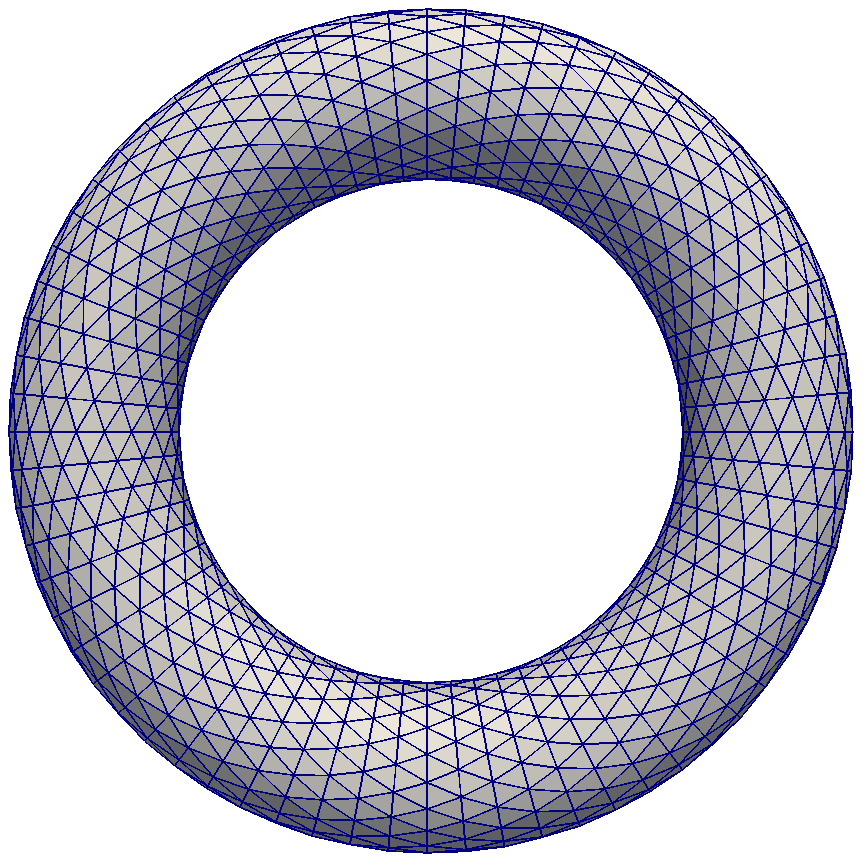
\includegraphics[width=\textwidth]{pic/torusgrid.png}
        \onslide<3> \centering\begin{tikzpicture}[>=latex, line width=1.5pt, scale=1.5]
  % Coords
\coordinate (V0) at (2,0);
\coordinate (V1) at (2,2);
\coordinate (V2) at (0,1);
\coordinate (V3) at (4,1);
\coordinate (V4) at (4,-1);
\coordinate (V5) at (0,-1);
\coordinate (V6) at (2,-2);

%circumcenter
\coordinate (CC1) at (1.333,1);
\coordinate (CC0) at (2.666,1);
\coordinate (CC3) at (1.333,-1);
\coordinate (CC2) at (0.666,0);
\coordinate (CC4) at (2.666,-1);
\coordinate (CC5) at (3.333,0);

 
\coordinate (C01) at (2,1);
\coordinate (C02) at (1,0.5);
\coordinate (C03) at (3,0.5);
\coordinate (C05) at (1,-0.5);
\coordinate (C04) at (3,-0.5);
\coordinate (C06) at (2,-1);

\coordinate (C12) at (1,1.5);
\coordinate (C25) at (0,0);
\coordinate (C56) at (1,-1.5);
\coordinate (C46) at (3,-1.5);
\coordinate (C34) at (4,0);
\coordinate (C13) at (3,1.5);

%\fill[black, opacity=0.2] (CC0) -- (CC1) -- (CC2) -- (CC3) -- (CC4) -- (CC5) -- (CC0);
%\fill[black, opacity=0.3] (V0) -- (CC5) -- (CC0) -- (V0);
%\fill[opacity=0.4]  (V1) -- (V3) -- (V4) -- (V6) -- (V5) -- (V2);
  % Arrows\tilde{\sigma}
\draw[->](V0) -- (V1);
\draw[<-](V1) --  (V2);
\draw[->](V0) -- (V2);
\draw[->](V1) --  (V3);
%\draw[blue,->](V0) -- (V3);
\draw[->](V0) -- (V3);
\draw[->](V0) -- (V4);
\draw[->](V0) -- (V5);
\draw[->](V5) --  (V2);
\draw[->](V3) --  (V4);
\draw[->](V4) -- (V6);
\draw[->](V0) -- (V6);
\draw[->](V6) -- (V5);
 
\draw[->] (CC0) + (135:0.2) arc (135:405:0.2) --++ (-3pt,3pt);
\draw[->] (CC1) + (135:0.2) arc (135:405:0.2) --++ (-3pt,3pt);
\draw[->] (CC2) + (135:0.2) arc (135:405:0.2) --++ (-3pt,3pt);
\draw[->] (CC3) + (135:0.2) arc (135:405:0.2) --++ (-3pt,3pt);
\draw[->] (CC4) + (135:0.2) arc (135:405:0.2) --++ (-3pt,3pt);
\draw[->] (CC5) + (135:0.2) arc (135:405:0.2) --++ (-3pt,3pt);


%\draw (CC0) -- (CC1) -- (CC2) -- (CC3) -- (CC4) -- (CC5) -- (CC0);
%\draw[dotted] (C12) -- (CC1);
%\draw[dotted] (C25) -- (CC2);
%\draw[dotted] (C56) -- (CC3);
%\draw[dotted] (C46) -- (CC4);
%\draw[dotted] (C34) -- (CC5);
%\draw[dotted] (C13) -- (CC0);
%\draw[dotted] (CC1) -- (CC4);
%\draw[dotted] (CC2) -- (CC5);
%\draw[dotted] (CC3) -- (CC0);
%
%\draw[dotted] (CC1) -- (V1);
%\draw[dotted] (CC2) -- (V2);
%\draw[dotted] (CC3) -- (V5);
%\draw[dotted] (CC4) -- (V6);
%\draw[dotted] (CC5) -- (V4);
%\draw[dotted] (CC0) -- (V3);
%
%\draw[dotted] (CC1) -- (V2);
%\draw[dotted] (CC2) -- (V5);
%\draw[dotted] (CC3) -- (V6);
%\draw[dotted] (CC4) -- (V4);
%\draw[dotted] (CC5) -- (V3);
%\draw[dotted] (CC0) -- (V1);

%\draw[blue,->] (CC5) -- (CC0); 

\fill[] (V0) circle (2pt);
%\fill[red] (V0) node[left] {\(v\ \)} circle (2pt);
\fill (V1) circle (2pt);
\fill (V2) circle (2pt);
\fill (V3) circle (2pt);
\fill (V4) circle (2pt);
\fill (V5)circle (2pt);
\fill (V6)circle (2pt);

%\fill (CC0) circle (2pt);
%\fill (CC1) circle (2pt);
%\fill (CC2) circle (2pt);
%\fill (CC3) circle (2pt);
%\fill (CC4) circle (2pt);
%\fill (CC5) circle (2pt);
%
%
%
%\fill (C01) circle (2pt);
%\fill (C02) circle (2pt);
%\fill (C03) node[right, blue] {\(\ e\)}circle (2pt);
%\fill (C05) circle (2pt);
%\fill (C04) circle (2pt);
%\fill (C06) circle (2pt);
% 
%
%\fill (C12) circle (2pt);
%\fill (C25) circle (2pt);
%\fill (C56) circle (2pt);
%\fill (C46) circle (2pt);
%\fill (C34) circle (2pt);
%\fill (C13) circle (2pt);


\end{tikzpicture}


        \onslide<4> \centering\begin{tikzpicture}[>=latex, line width=1.5pt, scale=1.5]
  % Coords
\coordinate (V0) at (2,0);
\coordinate (V1) at (2,2);
\coordinate (V2) at (0,1);
\coordinate (V3) at (4,1);
\coordinate (V4) at (4,-1);
\coordinate (V5) at (0,-1);
\coordinate (V6) at (2,-2);

%circumcenter
\coordinate (CC1) at (1.333,1);
\coordinate (CC0) at (2.666,1);
\coordinate (CC3) at (1.333,-1);
\coordinate (CC2) at (0.666,0);
\coordinate (CC4) at (2.666,-1);
\coordinate (CC5) at (3.333,0);

 
\coordinate (C01) at (2,1);
\coordinate (C02) at (1,0.5);
\coordinate (C03) at (3,0.5);
\coordinate (C05) at (1,-0.5);
\coordinate (C04) at (3,-0.5);
\coordinate (C06) at (2,-1);

\coordinate (C12) at (1,1.5);
\coordinate (C25) at (0,0);
\coordinate (C56) at (1,-1.5);
\coordinate (C46) at (3,-1.5);
\coordinate (C34) at (4,0);
\coordinate (C13) at (3,1.5);

\fill[black, opacity=0.3] (CC0) -- (CC1) -- (CC2) -- (CC3) -- (CC4) -- (CC5) -- (CC0);
%\fill[black, opacity=0.3] (V0) -- (CC5) -- (CC0) -- (V0);
%\fill[opacity=0.4]  (V1) -- (V3) -- (V4) -- (V6) -- (V5) -- (V2);
  % Arrows\tilde{\sigma}
\draw[->](V0) -- (V1);
\draw[<-](V1) --  (V2);
\draw[->](V0) -- (V2);
\draw[->](V1) --  (V3);
%\draw[blue,->](V0) -- (V3);
\draw[->](V0) -- (V3);
\draw[->](V0) -- (V4);
\draw[->](V0) -- (V5);
\draw[->](V5) --  (V2);
\draw[->](V3) --  (V4);
\draw[->](V4) -- (V6);
\draw[->](V0) -- (V6);
\draw[->](V6) -- (V5);
 
%\draw (CC0) -- (CC1) -- (CC2) -- (CC3) -- (CC4) -- (CC5) -- (CC0);
%\draw[dotted] (C12) -- (CC1);
%\draw[dotted] (C25) -- (CC2);
%\draw[dotted] (C56) -- (CC3);
%\draw[dotted] (C46) -- (CC4);
%\draw[dotted] (C34) -- (CC5);
%\draw[dotted] (C13) -- (CC0);
%\draw[dotted] (CC1) -- (CC4);
%\draw[dotted] (CC2) -- (CC5);
%\draw[dotted] (CC3) -- (CC0);
%
%\draw[dotted] (CC1) -- (V1);
%\draw[dotted] (CC2) -- (V2);
%\draw[dotted] (CC3) -- (V5);
%\draw[dotted] (CC4) -- (V6);
%\draw[dotted] (CC5) -- (V4);
%\draw[dotted] (CC0) -- (V3);
%
%\draw[dotted] (CC1) -- (V2);
%\draw[dotted] (CC2) -- (V5);
%\draw[dotted] (CC3) -- (V6);
%\draw[dotted] (CC4) -- (V4);
%\draw[dotted] (CC5) -- (V3);
%\draw[dotted] (CC0) -- (V1);

%\draw[blue,->] (CC5) -- (CC0); 

%\fill[] (V0) circle (2pt);
\fill[] (V0) node[left] {\(v\ \)} circle (2pt);
\fill (V1) circle (2pt);
\fill (V2) circle (2pt);
\fill (V3) circle (2pt);
\fill (V4) circle (2pt);
\fill (V5)circle (2pt);
\fill (V6)circle (2pt);

%\fill (CC0) circle (2pt);
%\fill (CC1) circle (2pt);
%\fill (CC2) circle (2pt);
%\fill (CC3) circle (2pt);
%\fill (CC4) circle (2pt);
%\fill (CC5) circle (2pt);
%
%
%
%\fill (C01) circle (2pt);
%\fill (C02) circle (2pt);
%\fill (C03) node[right, blue] {\(\ e\)}circle (2pt);
%\fill (C05) circle (2pt);
%\fill (C04) circle (2pt);
%\fill (C06) circle (2pt);
% 
%
%\fill (C12) circle (2pt);
%\fill (C25) circle (2pt);
%\fill (C56) circle (2pt);
%\fill (C46) circle (2pt);
%\fill (C34) circle (2pt);
%\fill (C13) circle (2pt);


\end{tikzpicture}


        \onslide<5> \centering\begin{tikzpicture}[>=latex, line width=1.5pt, scale=1.5]
  % Coords
\coordinate (V0) at (2,0);
\coordinate (V1) at (2,2);
\coordinate (V2) at (0,1);
\coordinate (V3) at (4,1);
\coordinate (V4) at (4,-1);
\coordinate (V5) at (0,-1);
\coordinate (V6) at (2,-2);

%circumcenter
\coordinate (CC1) at (1.333,1);
\coordinate (CC0) at (2.666,1);
\coordinate (CC3) at (1.333,-1);
\coordinate (CC2) at (0.666,0);
\coordinate (CC4) at (2.666,-1);
\coordinate (CC5) at (3.333,0);

 
\coordinate (C01) at (2,1);
\coordinate (C02) at (1,0.5);
\coordinate (C03) at (3,0.5);
\coordinate (C05) at (1,-0.5);
\coordinate (C04) at (3,-0.5);
\coordinate (C06) at (2,-1);

\coordinate (C12) at (1,1.5);
\coordinate (C25) at (0,0);
\coordinate (C56) at (1,-1.5);
\coordinate (C46) at (3,-1.5);
\coordinate (C34) at (4,0);
\coordinate (C13) at (3,1.5);

%\fill[black, opacity=0.3] (CC0) -- (CC1) -- (CC2) -- (CC3) -- (CC4) -- (CC5) -- (CC0);
%\fill[black, opacity=0.3] (V0) -- (CC5) -- (CC0) -- (V0);
%\fill[opacity=0.4]  (V1) -- (V3) -- (V4) -- (V6) -- (V5) -- (V2);
  % Arrows\tilde{\sigma}
\draw[->](V0) -- (V1);
\draw[<-](V1) --  (V2);
\draw[->](V0) -- (V2);
\draw[->](V1) --  (V3);
%\draw[blue,->](V0) -- (V3);
\draw[->](V0) -- (V3);
\draw[->](V0) -- (V4);
\draw[->](V0) -- (V5);
\draw[->](V5) --  (V2);
\draw[->](V3) --  (V4);
\draw[->](V4) -- (V6);
\draw[->](V0) -- (V6);
\draw[->](V6) -- (V5);
 
\begin{scope}[gray,  line width=1pt]
  \draw[->] (CC0) -- (CC1);
  \draw[->] (CC1) -- (CC2);
  \draw[->] (CC2) -- (CC3);
  \draw[->] (CC3) -- (CC4);
  \draw[->] (CC4) -- (CC5);
  \draw[->] (CC5) -- (CC0);
  \draw[<-,densely dotted] (C12) -- (CC1);
  \draw[<-,densely dotted] (C25) -- (CC2);
  \draw[<-,densely dotted] (C56) -- (CC3);
  \draw[<-,densely dotted] (C46) -- (CC4);
  \draw[<-,densely dotted] (C34) -- (CC5);
  \draw[<-,densely dotted] (C13) -- (CC0);
\fill (CC0) circle (1pt);
\fill (CC1) circle (1pt);
\fill (CC2) circle (1pt);
\fill (CC3) circle (1pt);
\fill (CC4) circle (1pt);
\fill (CC5) circle (1pt);



\fill (C01) circle (1pt);
\fill (C02) circle (1pt);
\fill (C03) circle (1pt);
\fill (C05) circle (1pt);
\fill (C04) circle (1pt);
\fill (C06) circle (1pt);
 

\fill (C12) circle (1pt);
\fill (C25) circle (1pt);
\fill (C56) circle (1pt);
\fill (C46) circle (1pt);
\fill (C34) circle (1pt);
\fill (C13) circle (1pt);
\end{scope}
%\draw[dotted] (CC1) -- (CC4);
%\draw[dotted] (CC2) -- (CC5);
%\draw[dotted] (CC3) -- (CC0);

%\draw[dotted] (CC1) -- (V1);
%\draw[dotted] (CC2) -- (V2);
%\draw[dotted] (CC3) -- (V5);
%\draw[dotted] (CC4) -- (V6);
%\draw[dotted] (CC5) -- (V4);
%\draw[dotted] (CC0) -- (V3);
%
%\draw[dotted] (CC1) -- (V2);
%\draw[dotted] (CC2) -- (V5);
%\draw[dotted] (CC3) -- (V6);
%\draw[dotted] (CC4) -- (V4);
%\draw[dotted] (CC5) -- (V3);
%\draw[dotted] (CC0) -- (V1);

%\draw[blue,->] (CC5) -- (CC0); 

\fill[] (V0) circle (2pt);
%\fill[] (V0) node[left] {\(v\ \)} circle (2pt);
\fill (V1) circle (2pt);
\fill (V2) circle (2pt);
\fill (V3) circle (2pt);
\fill (V4) circle (2pt);
\fill (V5)circle (2pt);
\fill (V6)circle (2pt);



\end{tikzpicture}


        \onslide<6> \centering\begin{tikzpicture}[>=latex, line width=1.5pt, scale=1.5]
  % Coords
\coordinate (V0) at (2,0);
\coordinate (V1) at (2,2);
\coordinate (V2) at (0,1);
\coordinate (V3) at (4,1);
\coordinate (V4) at (4,-1);
\coordinate (V5) at (0,-1);
\coordinate (V6) at (2,-2);

%circumcenter
\coordinate (CC1) at (1.333,1);
\coordinate (CC0) at (2.666,1);
\coordinate (CC3) at (1.333,-1);
\coordinate (CC2) at (0.666,0);
\coordinate (CC4) at (2.666,-1);
\coordinate (CC5) at (3.333,0);

 
\coordinate (C01) at (2,1);
\coordinate (C02) at (1,0.5);
\coordinate (C03) at (3,0.5);
\coordinate (C05) at (1,-0.5);
\coordinate (C04) at (3,-0.5);
\coordinate (C06) at (2,-1);

\coordinate (C12) at (1,1.5);
\coordinate (C25) at (0,0);
\coordinate (C56) at (1,-1.5);
\coordinate (C46) at (3,-1.5);
\coordinate (C34) at (4,0);
\coordinate (C13) at (3,1.5);

%\fill[black, opacity=0.3] (CC0) -- (CC1) -- (CC2) -- (CC3) -- (CC4) -- (CC5) -- (CC0);
%\fill[black, opacity=0.3] (V0) -- (CC5) -- (CC0) -- (V0);
%\fill[opacity=0.4]  (V1) -- (V3) -- (V4) -- (V6) -- (V5) -- (V2);
  % Arrows\tilde{\sigma}
\draw[->](V0) -- (V1);
\draw[<-](V1) --  (V2);
\draw[->](V0) -- (V2);
\draw[->](V1) --  (V3);
%\draw[blue,->](V0) -- (V3);
\draw[->](V0) -- (V3);
\draw[->](V0) -- (V4);
\draw[->](V0) -- (V5);
\draw[->](V5) --  (V2);
\draw[->](V3) --  (V4);
\draw[->](V4) -- (V6);
\draw[->](V0) -- (V6);
\draw[->](V6) -- (V5);
 
\begin{scope}[gray,  line width=1pt]
  %\draw[->] (CC0) -- (CC1);
  %\draw[->] (CC1) -- (CC2);
  %\draw[->] (CC2) -- (CC3);
  %\draw[->] (CC3) -- (CC4);
  %\draw[->] (CC4) -- (CC5);
  %\draw[->] (CC5) -- (CC0);
  %\draw[<-,densely dotted] (C12) -- (CC1);
  %\draw[<-,densely dotted] (C25) -- (CC2);
  %\draw[<-,densely dotted] (C56) -- (CC3);
  %\draw[<-,densely dotted] (C46) -- (CC4);
  %\draw[<-,densely dotted] (C34) -- (CC5);
  %\draw[<-,densely dotted] (C13) -- (CC0);
%\draw[dotted] (CC1) -- (CC4);
%\draw[dotted] (CC2) -- (CC5);
%\draw[dotted] (CC3) -- (CC0);

%\draw[dotted] (CC1) -- (V1);
%\draw[dotted] (CC2) -- (V2);
%\draw[dotted] (CC3) -- (V5);
%\draw[dotted] (CC4) -- (V6);
%\draw[dotted] (CC5) -- (V4);
%\draw[dotted] (CC0) -- (V3);
%
%\draw[dotted] (CC1) -- (V2);
%\draw[dotted] (CC2) -- (V5);
%\draw[dotted] (CC3) -- (V6);
%\draw[dotted] (CC4) -- (V4);
%\draw[dotted] (CC5) -- (V3);
%\draw[dotted] (CC0) -- (V1);

%\draw[blue,->] (CC5) -- (CC0); 

\fill (CC0) circle (2pt);
\fill (CC1) circle (2pt);
\fill (CC2) circle (2pt);
\fill (CC3) circle (2pt);
\fill (CC4) circle (2pt);
\fill (CC5) circle (2pt);

%
%
%\fill (C01) circle (2pt);
%\fill (C02) circle (2pt);
%\fill (C03) node[right, blue] {\(\ e\)}circle (2pt);
%\fill (C05) circle (2pt);
%\fill (C04) circle (2pt);
%\fill (C06) circle (2pt);
% 
%
%\fill (C12) circle (2pt);
%\fill (C25) circle (2pt);
%\fill (C56) circle (2pt);
%\fill (C46) circle (2pt);
%\fill (C34) circle (2pt);
%\fill (C13) circle (2pt);
\end{scope}

\fill[] (V0) circle (2pt);
%\fill[] (V0) node[left] {\(v\ \)} circle (2pt);
\fill (V1) circle (2pt);
\fill (V2) circle (2pt);
\fill (V3) circle (2pt);
\fill (V4) circle (2pt);
\fill (V5)circle (2pt);
\fill (V6)circle (2pt);



\end{tikzpicture}


        \onslide<7> \centering\begin{tikzpicture}[>=latex, line width=2pt, scale=2.7]
\usetikzlibrary{calc}

\edef\n{2}

\pgfmathparse{\n-1}
\edef\nmone{\pgfmathresult}

\pgfmathparse{\n-2}
\edef\nmtwo{\pgfmathresult}

%all the gray (dual) stuff
\begin{scope}[gray,  line width=1pt]
%dual vertices
\foreach \x in {0,...,\nmone} {
	\foreach \y in {0,...,\nmone} {
		\coordinate (V) at (\x+0.5,\y+0.5);
		\fill (V) circle(0.5pt);
	}
}

%dual x-edges
\foreach \x in {0,...,\nmtwo} {
	\foreach \y in {0,...,\nmone} {
		\coordinate (V1) at (\x+0.5,\y+0.5);
		\coordinate (V2) at (\x+1.5,\y+0.5); 
		\draw[<-] (V1) -- (V2);
	}
}

%dual y-edges
\foreach \x in {0,...,\nmone} {
	\foreach \y in {0,...,\nmtwo} {
		\coordinate (V1) at (\x+0.5,\y+0.5);
		\coordinate (V2) at (\x+0.5,\y+1.5); 
		\draw[->] (V1) -- (V2);
	}
}

%all remaining (half) dual edges on the boundaries 
\foreach \xy in {0,...,\nmone} {
	\draw[->,densely dotted] (\xy+0.5, 0) --  (\xy+0.5, 0.5); 
	\draw[->,densely dotted] (\xy+0.5, \n-0.5) --  (\xy+0.5, \n);
	\draw[<-,densely dotted] (0,\xy+0.5) -- (0.5,\xy+0.5);
	\draw[<-,densely dotted] (\n-0.5,\xy+0.5) -- (\n,\xy+0.5);
}
\end{scope}

%primal vertices
\foreach \x in {0,...,\n} {
	\foreach \y in {0,...,\n} {
		\coordinate (V) at (\x,\y);
		\fill (V) circle(1pt);
	}
}

%primal x-edges
\foreach \x in {0,...,\nmone} {
	\foreach \y in {0,...,\n} {
		\coordinate (V1) at (\x,\y);
		\coordinate (V2) at (\x+1,\y); 
		\draw[->] (V1) -- (V2);
	}
}

%primal y-edges
\foreach \x in {0,...,\n} {
	\foreach \y in {0,...,\nmone} {
		\coordinate (V1) at (\x,\y);
		\coordinate (V2) at (\x,\y+1); 
		\draw[->] (V1) -- (V2);
	}
}

%primal edge circumcenters
\foreach \xy in {0,...,\n} {
	\foreach \yx in {0,...,\nmone} {
		\coordinate (VX) at (\yx+0.5,\xy);
		\coordinate (VY) at (\xy,\yx+0.5);
		\fill (VX) circle(1pt);
		\fill (VY) circle(1pt);
	}
}

%%nodes
%\node[below right] at (1,1) {$v_{i,j}$};
%\node[below right] at (2,1) {$v_{i+1,j}$};
%
%\node[above right] at (1.5,1) {$e^x_{i,j}$};
%\node[above right] at (1.5,0) {$e^x_{i,j-1}$};
%\node[above right] at (1.5,2) {$e^x_{i,j+1}$};
%
%\node[below right] at (1,1.5) {$e^y_{i,j}$};
%\node[below right] at (2,1.5) {$e^y_{i+1,j}$};
%\node[below right] at (1,0.5) {$e^y_{i,j-1}$};
%\node[below right] at (2,0.5) {$e^y_{i+1,j-1}$};



\end{tikzpicture}

      \end{overprint}
    \end{minipage}
  \end{frame}

  \begin{frame}
    \nframetitle{Degrees Of Freedom (DOFs)}
    \begin{itemize}
      \item<1-> Discrete differential forms maps simplices to integral values over their.
      \item<2-> 0-form \( p_{h}\in\Lambda^{0}_{h}\SC \):\quad \( p_{h}(v) = \int_{\pi(v)}p = p(v) \)
      \item<3-> 1-form \( u_{h}\in\Lambda^{1}_{h}\SC \):\quad \( u_{h}(e) = \int_{\pi(e)}\ub\)
             \begin{itemize}
              \item<4-> \( u_{h}(e) \approx \ub(\mathbf{e}) = \left\langle \vb, \mathbf{e} \right\rangle \) on an intermediate point \(\xi\in\pi(e)\subset\surf  \).
             \end{itemize}
    \end{itemize}
  \end{frame}

  \begin{frame}
    \nframetitle{Discrete Hodge Operator}
    \begin{overprint}
    \onslide<1-6>
        \begin{itemize}
          \item<1-> \( p_{h}\in\Lambda^{0}_{h}\SC \),\quad  \( u_{h}\in\Lambda^{1}_{h}\SC \),\quad \( \omega_{h}\in\Lambda^{2}_{h}\SC \)
        \end{itemize}
        \begin{multicols}{2}
          \begin{itemize}
            \item<2-> \( (*p)_{h}(\face) \approx  \left|\face \right|p_{h}(\star\face) \)\vspace{1pt}
            \item<3-> \( (*\omega)_{h}(v) \approx  \frac{1}{\left| \star v \right|}\omega_{h}\left( \star v \right) \)\vspace{3pt}
            \item<4-> \( (*u)_{h}(e) \approx -\frac{\left| e \right|}{\left| \star e \right|}u_{h}(\star e) \)
          \end{itemize}
          \columnbreak
          \begin{itemize}
            \item<2-> \( (*p)_{h}(\star v) \approx  \left| \star v \right|p_{h}(v) \)
            \item<3-> \( (*\omega)_{h}(\star\face) \approx \frac{1}{\left| T \right|}\omega_{h}\left( T \right)\)
            \item<4-> \( (*u)_{h}(\star e) \approx \frac{\left| \star e \right|}{\left| e \right|}u_{h}(e) \)
          \end{itemize}
        \end{multicols}
        \begin{itemize}
          \item<5-> Many other ways to define a discrete Hodge star operator\footnotemark[1] 
        \end{itemize}
    \onslide<7> \centering\begin{tikzpicture}[>=latex, line width=2pt, scale=0.8]

% vertex coords
\coordinate (V1) at (0,-2);
\coordinate (V2) at (0,2);
\coordinate (V3) at (3,0);
\coordinate (V4) at (-3,0);

%points
\fill(V1) circle(2pt);
\fill(V2) circle(2pt);
\fill(V3) circle(2pt);
\fill(V4) circle(2pt);

%arrows
\draw[->] (V1) -- (V2) node [midway,left] {$e$} ;
\draw[->] (V2) -- (V3) node [midway,above] {$\tilde{e}_{2}$};
\draw[->] (V1) -- (V3) node [midway,below] {$\tilde{e}_{1}$};
\draw[->] (V4) -- (V2) node [midway,above] {$\tilde{e}_{3}$};
\draw[->] (V4) -- (V1) node [midway,below] {$\tilde{e}_{4}$};




\end{tikzpicture}

    \onslide<8>
        \begin{align}
          \begin{aligned}
        	\frac{1}{\tau_{k}}\ub_{k+1} + \exd q_{k+1} + (* \exd \ub_{k+1})({\color{altcol}* \ub_{k}}) - (*\exd * )&({\color{altcol}* \ub_{k}})({\color{altcol}* \ub_{k+1}}) \nonumber \\ 
        	- \frac{1}{\text{Re}} \left(  (*\exd * \exd) \ub_{k+1} + 2\gaussianCurvature \ub_{k+1} \right) &= \frac{1}{\tau_{k}}\ub_{k} + (* \exd\ub_{k})({\color{altcol}* \ub_{k}}) \\
        	{\color{altcol}\left\langle \ub_{k+1}, \ub_{k} \right\rangle} + p_{k+1} - q_{k+1} &= \frac{1}{2}{\color{altcol}\left\| \ub_{k} \right\|^{2}} \\
        	* \exd * \ub_{k+1} &= 0 
          \end{aligned}\tag{TDNSE}
        \end{align}
    \end{overprint}
    \vspace{-93pt}
    \begin{itemize}
      \item<6-> \eg\vspace{-25pt}
        \begin{align*}
        	\left( *\ub \right)_{h}(e) &\approx \circledast u_h(e) \\
        	&:= \frac{1}{4}\sum_{\face \succ e}\sum_{\substack{\tilde{e}\prec\face\\\tilde{e}\ne e}} \frac{s_{e\tilde{e}}}{\sqrt{\left| e \right|^{2}\left| \tilde{e} \right|^{2} - \left( \vect{e}\cdot\tilde{\vect{e}}\right)^{2}}} \left( \left( \vect{e}\cdot\tilde{\vect{e}} \right) u_h(e) -\left| e \right|^{2} u_h(\tilde{e}) \right)
        \end{align*}
    \vspace{-15pt}
    \end{itemize}
		\footnotetext[1]{\tiny\fullcite{Mohamed_CAD_2016}\vskip0pt}
  \end{frame}

  \begin{frame}
    \nframetitle{Operator Discretizations\footnotemark[1]}
    \begin{overprint}
      \onslide<1,7,10,13,15>
        \begin{align}
          \begin{aligned}
        	\frac{1}{\tau_{k}}\ub_{k+1} + \exd q_{k+1} 
              + \alt<7>{{\color{altcol}(* \exd \ub_{k+1})(* \ub_{k})}}{(* \exd \ub_{k+1})(* \ub_{k})} 
              -\alt<13>{{\color{altcol}(*\exd * )}}{(*\exd * )} & \alt<13>{{\color{altcol}(* \ub_{k})(* \ub_{k+1})}}{(* \ub_{k})(* \ub_{k+1})} \nonumber \\ 
        	    - \frac{1}{\text{Re}} \left(  \alt<1>{{\color{altcol}(*\exd * \exd) \ub_{k+1}}}{(*\exd * \exd) \ub_{k+1}} + 2\gaussianCurvature \ub_{k+1} \right) 
          &= \frac{1}{\tau_{k}}\ub_{k} + (* \exd\ub_{k})(* \ub_{k}) \\
        	\alt<15>{{\color{altcol}\left\langle \ub_{k+1}, \ub_{k} \right\rangle}}{\left\langle \ub_{k+1}, \ub_{k} \right\rangle} + p_{k+1} - q_{k+1} &= \frac{1}{2}\left\| \ub_{k} \right\|^{2} \\
        	\alt<10>{{\color{altcol}* \exd * \ub_{k+1}}}{* \exd * \ub_{k+1}} &= 0 
          \end{aligned}\tag{TDNSE}
        \end{align}
      \onslide<2> \centering\begin{tikzpicture}[>=latex, line width=2pt, scale=0.8]

%define picture size
\draw[opacity=0] (-3.1,-2.1) rectangle (3.1,2.3);

% vertex coords
\coordinate (V1) at (0,-2);
\coordinate (V2) at (0,2);
\coordinate (V3) at (3,0);
\coordinate (V4) at (-3,0);

%Circumcenters
\coordinate (CC1) at (-0.833,0);
\coordinate (CC2) at (0.833,0);
\draw[->,gray] (CC2) -- (CC1) node [midway,below right]{$\star e$};

%points
\fill(V1) circle(2pt);
\fill(V2) circle(2pt);
\fill(V3) circle(2pt);
\fill(V4) circle(2pt);

\fill[gray] (CC1) circle(2pt);
\fill[gray] (CC2) circle(2pt);

\node[left] at (CC1) {$T_{1}$};
\node[right] at (CC2) {$T_{2}$};


%arrows
\draw[->] (V1) -- (V2) node [midway,above left] {$e$} ;
\draw[<-] (V2) -- (V3) node [midway,above] {$\tilde{e}_{2}$};
\draw[->] (V1) -- (V3) node [midway,below] {$\tilde{e}_{1}$};
\draw[->] (V4) -- (V2) node [midway,above] {$\tilde{e}_{3}$};
\draw[<-] (V4) -- (V1) node [midway,below] {$\tilde{e}_{4}$};







\end{tikzpicture}

      \onslide<3> \centering\begin{tikzpicture}[>=latex, line width=2pt, scale=0.8]

% vertex coords
\coordinate (V1) at (0,-2);
\coordinate (V2) at (0,2);
\coordinate (V3) at (3,0);
\coordinate (V4) at (-3,0);

%points
\fill(V1) circle(2pt);
\fill(V2) circle(2pt);
\fill(V3) circle(2pt);
\fill(V4) circle(2pt);

%arrows
\draw[->] (V1) -- (V2) node [midway,left=-35pt] {$-\frac{\left| e \right|}{\left| \star e \right|}\left(\frac{1}{\left|T_{1} \right|} +\frac{1}{\left|T_{2} \right|} \right)$} ;
\draw[<-] (V2) -- (V3) node [midway,above=5pt] {$\frac{\left| e \right|}{\left| \star e \right|\left|T_{2} \right|}$};
\draw[->] (V1) -- (V3) node [midway,below] {$\frac{\left| e \right|}{\left| \star e \right|\left|T_{2} \right|}$};
\draw[->] (V4) -- (V2) node [midway,above=5pt] {$\frac{\left| e \right|}{\left| \star e \right|\left|T_{1} \right|}$};
\draw[<-] (V4) -- (V1) node [midway,below] {$\frac{\left| e \right|}{\left| \star e \right|\left|T_{2} \right|}$};

%define picture size
\draw[opacity=0] (-3.1,-2.1) rectangle (3.1,2.3);


\end{tikzpicture}

      \onslide<4-5> \centering\begin{tikzpicture}[>=latex, line width=2pt, scale=0.8]

%define picture size
\draw[opacity=0] (-4.1,-2.1) rectangle (5.5,3);

\coordinate (V0) at (0,-2);
\coordinate (V1) at (4,-2);
\coordinate (V2) at (4,2);
\coordinate (V3) at (0,2);
\coordinate (V4) at (-4,2);
\coordinate (V5) at (-4,-2);

\coordinate (C0) at (0,0);
\coordinate (C1) at (2,-2);
\coordinate (C2) at (4,0);
\coordinate (C3) at (2,2);
\coordinate (C4) at (-2,2);
\coordinate (C5) at (-4,0);
\coordinate (C6) at (-2,-2);

\coordinate (CC0) at (-2,0);
\coordinate (CC1) at (2,0);

\draw (V0) circle(2pt);
\draw (V1) circle(2pt);
\draw (V2) circle(2pt);
\draw (V3) circle(2pt);
\draw (V4) circle(2pt);
\draw (V5) circle(2pt);


\draw (C1) node[above right]{$u^x_{i,j}$} circle(2pt);
\draw (C2) node[above right]{$u^y_{i+1,j}$} circle(2pt);
\draw (C3) node[above right]{$u^x_{i,j+1}$} circle(2pt);
\draw (C4) node[above right]{$u^x_{i-1,j+1}$} circle(2pt);
\draw (C5) node[above right]{$u^y_{i-1,j}$} circle(2pt);
\draw (C6) node[above right]{$u^x_{i-1,j}$} circle(2pt);

\draw[gray] (CC0) circle(2pt);
\draw[gray] (CC1) circle(2pt);

\draw[->,gray] (CC1) -- (CC0);

\draw[->,gray,densely dotted] (C2) -- (CC1);
\draw[->,gray,densely dotted] (CC1) -- (C3);
\draw[->,gray,densely dotted] (CC0) -- (C4);
\draw[->,gray,densely dotted] (CC0) -- (C5);
\draw[->,gray,densely dotted] (C6) -- (CC0);
\draw[->,gray,densely dotted] (C1) -- (CC1);

\draw[->] (V0) -- (V3);
\draw[->] (V0) -- (V1);
\draw[->] (V1) -- (V2);
\draw[->] (V3) -- (V2);
\draw[->] (V4) -- (V3);
\draw[->] (V5) -- (V4);
\draw[->] (V5) -- (V0);

\draw (C0) node[above right]{$u^y_{i,j}$} circle(2pt);


\end{tikzpicture}

      \onslide<6> \centering\begin{tikzpicture}[>=latex, line width=2pt, scale=0.8]

%define picture size
\draw[opacity=0] (-4.1,-2.1) rectangle (5.5,3);

\coordinate (V0) at (0,-2);
\coordinate (V1) at (4,-2);
\coordinate (V2) at (4,2);
\coordinate (V3) at (0,2);
\coordinate (V4) at (-4,2);
\coordinate (V5) at (-4,-2);

\coordinate (C0) at (0,0);
\coordinate (C1) at (2,-2);
\coordinate (C2) at (4,0);
\coordinate (C3) at (2,2);
\coordinate (C4) at (-2,2);
\coordinate (C5) at (-4,0);
\coordinate (C6) at (-2,-2);

\coordinate (CC0) at (-2,0);
\coordinate (CC1) at (2,0);

\draw (V0) circle(2pt);
\draw (V1) circle(2pt);
\draw (V2) circle(2pt);
\draw (V3) circle(2pt);
\draw (V4) circle(2pt);
\draw (V5) circle(2pt);


\draw (C1) node[above right]{$-\frac{1}{h^{2}}$} circle(2pt);
\draw (C2) node[above right]{$+\frac{1}{h^{2}}$} circle(2pt);
\draw (C3) node[above right]{$+\frac{1}{h^{2}}$} circle(2pt);
\draw (C4) node[above right]{$-\frac{1}{h^{2}}$} circle(2pt);
\draw (C5) node[above right]{$+\frac{1}{h^{2}}$} circle(2pt);
\draw (C6) node[above right]{$+\frac{1}{h^{2}}$} circle(2pt);

%\draw[gray] (CC0) circle(2pt);
%\draw[gray] (CC1) circle(2pt);

%\draw[->,gray] (CC1) -- (CC0);

%\draw[->,gray,densely dotted] (C2) -- (CC1);
%\draw[->,gray,densely dotted] (CC1) -- (C3);
%\draw[->,gray,densely dotted] (CC0) -- (C4);
%\draw[->,gray,densely dotted] (CC0) -- (C5);
%\draw[->,gray,densely dotted] (C6) -- (CC0);
%\draw[->,gray,densely dotted] (C1) -- (CC1);

\draw[->] (V0) -- (V3);
\draw[->] (V0) -- (V1);
\draw[->] (V1) -- (V2);
\draw[->] (V3) -- (V2);
\draw[->] (V4) -- (V3);
\draw[->] (V5) -- (V4);
\draw[->] (V5) -- (V0);

\draw (C0) node[above right]{$-\frac{2}{h^{2}}$} circle(2pt);


\end{tikzpicture}

      \onslide<8> \centering\begin{tikzpicture}[>=latex, line width=2pt, scale=0.8]

%define picture size
\draw[opacity=0] (-3.1,-2.1) rectangle (3.1,2.3);

% vertex coords
\coordinate (V1) at (0,-2);
\coordinate (V2) at (0,2);
\coordinate (V3) at (3,0);
\coordinate (V4) at (-3,0);

%Circumcenters
\coordinate (CC1) at (-0.833,0);
\coordinate (CC2) at (0.833,0);
%\draw[->,gray] (CC2) -- (CC1) node [midway,below right]{$\star e$};

%points
\fill(V1) circle(2pt);
\fill(V2) circle(2pt);
\fill(V3) circle(2pt);
\fill(V4) circle(2pt);

%\fill[gray] (CC1) circle(2pt);
%\fill[gray] (CC2) circle(2pt);

\node[left] at (CC1) {$T_{1}$};
\node[right] at (CC2) {$T_{2}$};


%arrows
\draw[->] (V1) -- (V2) node [midway,above left] {$e$} ;
\draw[<-] (V2) -- (V3) node [midway,above] {$\tilde{e}_{2}$};
\draw[->] (V1) -- (V3) node [midway,below] {$\tilde{e}_{1}$};
\draw[<-] (V4) -- (V2) node [midway,above] {$\tilde{e}_{3}$};
\draw[->] (V4) -- (V1) node [midway,below] {$\tilde{e}_{4}$};







\end{tikzpicture}

      \onslide<9> \centering\begin{tikzpicture}[>=latex, line width=2pt, scale=0.8]

%define picture size
\draw[opacity=0] (-3.1,-2.1) rectangle (3.1,2.3);

% vertex coords
\coordinate (V1) at (0,-2);
\coordinate (V2) at (0,2);
\coordinate (V3) at (3,0);
\coordinate (V4) at (-3,0);

%Circumcenters
\coordinate (CC1) at (-0.833,0);
\coordinate (CC2) at (0.833,0);
%\draw[->,gray] (CC2) -- (CC1) node [midway,below right]{$\star e$};

%points
\fill(V1) circle(2pt);
\fill(V2) circle(2pt);
\fill(V3) circle(2pt);
\fill(V4) circle(2pt);

%\fill[gray] (CC1) circle(2pt);
%\fill[gray] (CC2) circle(2pt);

%\node[left] at (CC1) {$T_{1}$};
%\node[right] at (CC2) {$T_{2}$};


%arrows
\draw[->] (V1) -- (V2) node [midway,above left] {$0$} ;
\draw[<-] (V2) -- (V3) node [midway,above right=-5pt] {$\frac{(*u_k)_h(e)}{|T_1|+|T_2|}$};
\draw[->] (V1) -- (V3) node [midway,below right=-5pt] {$\frac{(*u_k)_h(e)}{|T_1|+|T_2|}$};
\draw[<-] (V4) -- (V2) node [midway,above left=-5pt] {$\frac{(*u_k)_h(e)}{|T_1|+|T_2|}$};
\draw[->] (V4) -- (V1) node [midway,below left=-5pt] {$\frac{(*u_k)_h(e)}{|T_1|+|T_2|}$};







\end{tikzpicture}

      \onslide<11,16> \centering\begin{tikzpicture}[>=latex, line width=2pt, scale=1]
  % Coords
\coordinate (V0) at (2,0);
\coordinate (V1) at (2,2);
\coordinate (V2) at (0,1);
\coordinate (V3) at (4,1);
\coordinate (V4) at (4,-1);
\coordinate (V5) at (0,-1);
\coordinate (V6) at (2,-2);

%circumcenter
\coordinate (CC1) at (1.333,1);
\coordinate (CC0) at (2.666,1);
\coordinate (CC3) at (1.333,-1);
\coordinate (CC2) at (0.666,0);
\coordinate (CC4) at (2.666,-1);
\coordinate (CC5) at (3.333,0);

 
\coordinate (C01) at (2,1);
\coordinate (C02) at (1,0.5);
\coordinate (C03) at (3,0.5);
\coordinate (C05) at (1,-0.5);
\coordinate (C04) at (3,-0.5);
\coordinate (C06) at (2,-1);

\coordinate (C12) at (1,1.5);
\coordinate (C25) at (0,0);
\coordinate (C56) at (1,-1.5);
\coordinate (C46) at (3,-1.5);
\coordinate (C34) at (4,0);
\coordinate (C13) at (3,1.5);

\begin{scope}[gray,  line width=1pt]
  \draw[->] (CC0) -- (CC1);
  \draw[->] (CC1) -- (CC2);
  \draw[->] (CC2) -- (CC3);
  \draw[->] (CC3) -- (CC4);
  \draw[->] (CC4) -- (CC5);
  \draw[->] (CC5) -- (CC0);
  \draw[<-,densely dotted] (C12) -- (CC1);
  \draw[<-,densely dotted] (C25) -- (CC2);
  \draw[<-,densely dotted] (C56) -- (CC3);
  \draw[<-,densely dotted] (C46) -- (CC4);
  \draw[<-,densely dotted] (C34) -- (CC5);
  \draw[<-,densely dotted] (C13) -- (CC0);
\fill (CC0) circle (1pt);
\fill (CC1) circle (1pt);
\fill (CC2) circle (1pt);
\fill (CC3) circle (1pt);
\fill (CC4) circle (1pt);
\fill (CC5) circle (1pt);



\fill (C01) circle (1pt);
\fill (C02) circle (1pt);
\fill (C03) circle (1pt);
\fill (C05) circle (1pt);
\fill (C04) circle (1pt);
\fill (C06) circle (1pt);
 

\fill (C12) circle (1pt);
\fill (C25) circle (1pt);
\fill (C56) circle (1pt);
\fill (C46) circle (1pt);
\fill (C34) circle (1pt);
\fill (C13) circle (1pt);
\end{scope}

%\fill[black, opacity=0.3] (CC0) -- (CC1) -- (CC2) -- (CC3) -- (CC4) -- (CC5) -- (CC0);
%\fill[black, opacity=0.3] (V0) -- (CC5) -- (CC0) -- (V0);
%\fill[opacity=0.4]  (V1) -- (V3) -- (V4) -- (V6) -- (V5) -- (V2);
  % Arrows\tilde{\sigma}
\draw[->](V0) -- (V1) node[midway,above right]{$\tilde{e}_1$};
\draw[<-](V1) --  (V2);
\draw[->](V0) -- (V2) node[midway,above]{$\tilde{e}_2$};
\draw[->](V1) --  (V3);
%\draw[blue,->](V0) -- (V3);
\draw[->](V0) -- (V3) node[midway,below]{$\tilde{e}_6$};
\draw[->](V0) -- (V4) node[midway,below]{$\tilde{e}_5$};
\draw[->](V0) -- (V5) node[midway,above]{$\tilde{e}_3$};
\draw[->](V5) --  (V2);
\draw[->](V3) --  (V4);
\draw[->](V4) -- (V6);
\draw[->](V0) -- (V6) node[midway,below left]{$\tilde{e}_5$};
\draw[->](V6) -- (V5);
 

%\draw[dotted] (CC1) -- (CC4);
%\draw[dotted] (CC2) -- (CC5);
%\draw[dotted] (CC3) -- (CC0);

%\draw[dotted] (CC1) -- (V1);
%\draw[dotted] (CC2) -- (V2);
%\draw[dotted] (CC3) -- (V5);
%\draw[dotted] (CC4) -- (V6);
%\draw[dotted] (CC5) -- (V4);
%\draw[dotted] (CC0) -- (V3);
%
%\draw[dotted] (CC1) -- (V2);
%\draw[dotted] (CC2) -- (V5);
%\draw[dotted] (CC3) -- (V6);
%\draw[dotted] (CC4) -- (V4);
%\draw[dotted] (CC5) -- (V3);
%\draw[dotted] (CC0) -- (V1);

%\draw[blue,->] (CC5) -- (CC0); 

\fill[] (V0) node[left] {\(v\ \)} circle (2pt);
\fill (V1) circle (2pt);
\fill (V2) circle (2pt);
\fill (V3) circle (2pt);
\fill (V4) circle (2pt);
\fill (V5)circle (2pt);
\fill (V6)circle (2pt);



\end{tikzpicture}


      \onslide<12> \centering\begin{tikzpicture}[>=latex, line width=2pt, scale=1]
  % Coords
\coordinate (V0) at (2,0);
\coordinate (V1) at (2,2);
\coordinate (V2) at (0,1);
\coordinate (V3) at (4,1);
\coordinate (V4) at (4,-1);
\coordinate (V5) at (0,-1);
\coordinate (V6) at (2,-2);

%circumcenter
\coordinate (CC1) at (1.333,1);
\coordinate (CC0) at (2.666,1);
\coordinate (CC3) at (1.333,-1);
\coordinate (CC2) at (0.666,0);
\coordinate (CC4) at (2.666,-1);
\coordinate (CC5) at (3.333,0);

 
\coordinate (C01) at (2,1);
\coordinate (C02) at (1,0.5);
\coordinate (C03) at (3,0.5);
\coordinate (C05) at (1,-0.5);
\coordinate (C04) at (3,-0.5);
\coordinate (C06) at (2,-1);

\coordinate (C12) at (1,1.5);
\coordinate (C25) at (0,0);
\coordinate (C56) at (1,-1.5);
\coordinate (C46) at (3,-1.5);
\coordinate (C34) at (4,0);
\coordinate (C13) at (3,1.5);

\fill[black, opacity=0.3] (CC0) -- (CC1) -- (CC2) -- (CC3) -- (CC4) -- (CC5) -- (CC0);
%\fill[black, opacity=0.3] (V0) -- (CC5) -- (CC0) -- (V0);
%\fill[opacity=0.4]  (V1) -- (V3) -- (V4) -- (V6) -- (V5) -- (V2);
  % Arrows\tilde{\sigma}
\draw[->](V0) -- (V1);
%\draw[<-](V1) --  (V2);
\draw[->](V0) -- (V2);
%\draw[->](V1) --  (V3);
%\draw[blue,->](V0) -- (V3);
\draw[->](V0) -- (V3);
\draw[->](V0) -- (V4);
\draw[->](V0) -- (V5);
%\draw[->](V5) --  (V2);
%\draw[->](V3) --  (V4);
%\draw[->](V4) -- (V6);
\draw[->](V0) -- (V6);
%\draw[->](V6) -- (V5);
 
%\draw (CC0) -- (CC1) -- (CC2) -- (CC3) -- (CC4) -- (CC5) -- (CC0);
%\draw[dotted] (C12) -- (CC1);
%\draw[dotted] (C25) -- (CC2);
%\draw[dotted] (C56) -- (CC3);
%\draw[dotted] (C46) -- (CC4);
%\draw[dotted] (C34) -- (CC5);
%\draw[dotted] (C13) -- (CC0);
%\draw[dotted] (CC1) -- (CC4);
%\draw[dotted] (CC2) -- (CC5);
%\draw[dotted] (CC3) -- (CC0);
%
%\draw[dotted] (CC1) -- (V1);
%\draw[dotted] (CC2) -- (V2);
%\draw[dotted] (CC3) -- (V5);
%\draw[dotted] (CC4) -- (V6);
%\draw[dotted] (CC5) -- (V4);
%\draw[dotted] (CC0) -- (V3);
%
%\draw[dotted] (CC1) -- (V2);
%\draw[dotted] (CC2) -- (V5);
%\draw[dotted] (CC3) -- (V6);
%\draw[dotted] (CC4) -- (V4);
%\draw[dotted] (CC5) -- (V3);
%\draw[dotted] (CC0) -- (V1);

%\draw[blue,->] (CC5) -- (CC0); 

%\fill[] (V0) circle (2pt);
\fill[] (V0) node[left] {\(v\ \)} circle (2pt);
\fill[opacity=0] (V1) circle (2pt);
%\fill (V2) circle (2pt);
%\fill (V3) circle (2pt);
%\fill (V4) circle (2pt);
%\fill (V5)circle (2pt);
%\fill (V6)circle (2pt);

%\fill (CC0) circle (2pt);
%\fill (CC1) circle (2pt);
%\fill (CC2) circle (2pt);
%\fill (CC3) circle (2pt);
%\fill (CC4) circle (2pt);
%\fill (CC5) circle (2pt);
%
%
%
%\fill (C01) circle (2pt);
%\fill (C02) circle (2pt);
%\fill (C03) node[right, blue] {\(\ e\)}circle (2pt);
%\fill (C05) circle (2pt);
%\fill (C04) circle (2pt);
%\fill (C06) circle (2pt);
% 
%
%\fill (C12) circle (2pt);
%\fill (C25) circle (2pt);
%\fill (C56) circle (2pt);
%\fill (C46) circle (2pt);
%\fill (C34) circle (2pt);
%\fill (C13) circle (2pt);


\end{tikzpicture}


      \onslide<14> \centering\begin{tikzpicture}[>=latex, line width=2pt, scale=1]
  % Coords
\coordinate (V0) at (0,2);
\coordinate (V1) at (2,2);
\coordinate (V2) at (1,0);
\coordinate (V3) at (1,4);
\coordinate (V4) at (-1,4);
\coordinate (V5) at (-1,0);
\coordinate (V6) at (-2,2);

%circumcenter
\coordinate (CC1) at (1,1.333);
\coordinate (CC0) at (1,2.666);
\coordinate (CC3) at (-1,1.333);
\coordinate (CC2) at (0,0.666);
\coordinate (CC4) at (-1,2.666);
\coordinate (CC5) at (0,3.333);

 % Coords
\coordinate (VS0) at (2,2);
\coordinate (VS1) at (4,2);
\coordinate (VS2) at (3,0);
\coordinate (VS3) at (3,4);
\coordinate (VS4) at (1,4);
\coordinate (VS5) at (1,0);
\coordinate (VS6) at (0,2);

%circumcenter
\coordinate (CCS1) at (3,1.333);
\coordinate (CCS0) at (3,2.666);
\coordinate (CCS3) at (1,1.333);
\coordinate (CCS2) at (2,0.666);
\coordinate (CCS4) at (1,2.666);
\coordinate (CCS5) at (2,3.333);

\fill[black, opacity=0.3] (CC0) -- (CC1) -- (CC2) -- (CC3) -- (CC4) -- (CC5) -- (CC0);
\fill[black, opacity=0.3] (CCS0) -- (CCS1) -- (CCS2) -- (CCS3) -- (CCS4) -- (CCS5) -- (CCS0);

\draw[->](V0) -- (V1) node[midway, above]{$e$};
\draw[->](V0) -- (V2);
\draw[->](V0) -- (V3);
\draw[->](V0) -- (V4);
\draw[->](V0) -- (V5);
\draw[->](V0) -- (V6);

\draw[->](VS0) -- (VS1);
\draw[->](VS0) -- (VS2);
\draw[->](VS0) -- (VS3);
\draw[->](VS0) -- (VS4);
\draw[->](VS0) -- (VS5);
%\draw[->](VS0) -- (VS6);


\fill[] (V0) node[above left] {\(v_1\ \)} circle (2pt);
\fill[] (VS0) node[above right] {\(\ v_2\)} circle (2pt);




\end{tikzpicture}


    \end{overprint}
    \vspace{-100pt}
    \begin{overprint}
      \onslide<1-4>
        \begin{align*}
          ( *\exd * \exd \ub_{k+1})_{h} (e) &\approx -\frac{\left| e \right|}{\left| \star e \right|} \sum_{\face\succ e} \frac{s_{\face,e}}{\left| \face \right|} \sum_{\tilde{e}\prec\face}
          s_{\face,\tilde{e}}\, (\ub_{k+1})_{h}(\tilde{e})
          =: ( *\exd * \exd)_{h} (\ub_{k+1})_{h} (e)
        \end{align*}
      \onslide<5-6>
        \begin{align*}
          (\Rot\Rot u)^{y}_{i,j} &=
	          \frac{1}{h^{2}}\left(  - 2u^{y}_{i,j} + u^{y}_{i+1,j} +  u^{y}_{i-1,j}
						-u^{x}_{i,j} + u^{x}_{i,j+1}
						-u^{x}_{i-1,j+1} +u^{x}_{i-1,j} \right) + \landau(h^{2})
        \end{align*}
      \onslide<7-9>
        \begin{align*}
          \left((* \exd \ub_{k+1})(*\ub_{k})\right)_{h}(e) &\approx \frac{(*\ub_{k})_{h}(e)}{\sum_{\face\succ e}|\face|}
          \sum_{\face\succ e}\sum_{\tilde{e}\prec\face}s_{\face,\tilde{e}}(\ub_{k+1})_{h}(\tilde{e})
            =:((* \ub_{k})(* \exd ))_{h}(\ub_{k+1})_{h}
        \end{align*}
      \onslide<10-12>
          \begin{align*}
            (*\exd * \ub_{k+1})_{h}(v) &\approx -\frac{1}{|\star v|}\sum_{\tilde{e}\succ v}s_{v,\tilde{e}}\frac{|\star \tilde{e}|}{|\tilde{e}|}(\ub_{k+1})_{h}(\tilde{e})
              =: (*\exd *)_{h} (\ub_{k+1})_{h}(v)
          \end{align*}
      \onslide<13>
        \begin{align*}
          \left((*\exd * )(*\ub_{k})(* \ub_{k+1})\right)_{h}(e) &\approx -\frac{1}{2}\left( \sum_{v\prec e} \frac{1}{|\star v|}\sum_{\tilde{e}\succ v}
                        s_{v,\tilde{e}}\frac{|\star \tilde{e}|}{|\tilde{e}|}(*\ub_{k})_{h}(\tilde{e}) \right) (*\ub_{k+1})_{h}(e)
        \end{align*}
      \onslide<14>
        \begin{align*}
          \hspace{-10pt}
          \left((*\exd * )(*\ub_{k})(* \ub_{k+1})\right)_{h}(e) &\approx \frac{1}{2}\left( \sum_{v\prec e} (*\exd*)_{h}(*\ub_{k})_{h}(v)\right) (*\ub_{k+1})_{h}(e)
              =: ((*\exd * )(* \ub_{k}))_{h}(* \ub_{k+1})_{h}
        \end{align*}
      \onslide<15-16>
        \begin{align*}
          \left\langle \ub_{k+1} , \ub_{k} \right\rangle_{h}(v)
              &\approx \frac{1}{4\left| \star v \right|}\sum_{\tilde{e}\succ v} 
              \frac{\left| \star \tilde{e} \right|}{\left| \tilde{e} \right|} \left( (\ub_{k})_{h}(\tilde{e}) (\ub_{k+1})_{h}(\tilde{e}) 
                                                          + \left( *\ub_{k} \right)_{h}(\tilde{e}) \left( *\ub_{k+1} \right)_{h}(\tilde{e}) \right)
        \end{align*}
    \end{overprint}
    \footnotetext[1]{\tiny\fullcite{nitschke_etal_2016}\vskip0pt}
  \end{frame}

  \begin{frame}
    \nframetitle{Fully-discrete equations}
    \begin{itemize}
      \item 
          For \( k=0,1,\ldots \) and given initial values \((\ub_{0})_{h}  \) and \((* \ub_{0})_{h}  \), 
          find \( (\ub_{k+1})_{h}, (* \ub_{k+1})_{h} \in \Lambda^{1}_{h}\SC \) and \( (p_{k+1})_{h},(q_{k+1})_{h}\in \Lambda^{0}_{h}\SC  \) s.t.
    \end{itemize}
    \begin{align}
      \begin{aligned}
      \circledast(\ub_{k+1})_{h} - (* \ub_{k+1})_{h} &= 0 &&\text{in } \Es\\
    	\frac{1}{\tau_{k}}(\ub_{k+1})_{h} + (\exd q_{k+1})_{h} 
          + ((* \ub_{k})(* \exd ))_{h}(\ub_{k+1})_{h} 
          &- ((*\exd * )(* \ub_{k}))_{h}(* \ub_{k+1})_{h} \nonumber \\ 
    	- \frac{1}{\text{Re}} \left(  (*\exd * \exd)_{h} (\ub_{k+1})_{h} + 2\gaussianCurvature (\ub_{k+1})_{h} \right) 
                    &= \frac{1}{\tau_{k}}(\ub_{k})_{h} + ((* \ub_{k})(* \exd ))_{h}(\ub_{k})_{h}  &&\text{in } \Es \\
    	\left\langle \cdot, \ub_{k} \right\rangle_{h}\left[ (\ub_{k+1})_{h}, (*\ub_{k+1})_{h} \right] 
            + (p_{k+1})_{h} - (q_{k+1})_{h} &= \left\langle \cdot, \ub_{k} \right\rangle_{h}\left[ (\ub_{k})_{h}, (*\ub_{k})_{h} \right] &&\text{in } \Vs\\
    	(* \exd *)_{h} (\ub_{k+1})_{h} &= 0 &&\text{in } \Vs
      \end{aligned}\tag{DECNSE}
    \end{align}
  \end{frame}
	
	\section{Eins}
	\begin{frame}
		\nframetitle{Content}
		\tableofcontents[current]
	\end{frame}
	\begin{frame}
		\nframetitle{Experimental Setup}
		\vskip20pt
		\begin{center}
			\begin{minipage}{0.41\textwidth}
				\begin{itemize}
					\item Experiment and Model\footnotemark[1]
					\item Shear flow through chamber
					\item Qualitative and quantitative results
				\end{itemize}
			\end{minipage}
			\hfill
			\begin{minipage}{0.55\textwidth}
				\centering
				\insertpicture{\textwidth}{pic/test.png}
			\end{minipage}
		\end{center}
		\vskip10pt
		\footnotetext[1]{\tiny\fullcite{HonerkampSmith_PRL_2013}\vskip0pt}
	\end{frame}
	
	\section{Zwei}
	\begin{frame}
		\nframetitle{Content}
		\tableofcontents[current]
	\end{frame}
	\begin{frame}
		\nframetitle{}
		\vskip20pt
	\end{frame}
	
	\section{Drei}
	\begin{frame}
		\nframetitle{Content}
		\tableofcontents[current]
	\end{frame}
	\begin{frame}
		\nframetitle{}
		\vskip20pt
	\end{frame}
	
	\section*{}
\begin{frame}
	\nframetitle{}
	\begin{center}
		\vfill
		\Large\textbf{Thank you for your attention!}
		\vfill
	\end{center}
\end{frame}
\end{document}


